\label{boolean_chapter}
\newtheorem{theorem}{Theorem}[chapter]

%\section{Cellular Automata}
%We begin discussing the cellular automata model, also called finite automata, finite state machine, etc. This %model is a particular case of a more general model called random Boolean network which we will introduce in the %next section. 

This chapter will be devoted to an introduction of Random Boolean Networks. First, we will begin by defining what a Boolean Network is, then we will present the Random Boolean Network Model. We will talk about the topology of these networks and the updating functions used. We will continue by discussing the dynamics of Random Boolean Networks and we will present an example. Afterward, we will briefly review the different dynamical phases and other possible updating schemes. We will finish by commenting on some applications and the software available to simulate Random Boolean Networks.\\

The model we are interested in was originally proposed by Stuart Kauffman in 1969 \cite{kauffman1} \cite{kauffman2}. He proposed a mathematical model to simulate genetic regulatory networks in which each gene was represented by a node which can only take the two values $0$ or $1$, i.e., every gene could only be in an "on" state or in an "off" state. There are $N$ nodes in the network, and the state of each node is controlled by the information it receives from $k$ randomly\footnote{It is supposed that we are using some probability distribution which can be for example a normal distribution.} chosen nodes (itself included) which are connected to it. Once the connections are established in a random way, they stay fixed during the dynamics of the network. Each node has associated with it one updating function which is also chosen in a random way from the set of all possible Boolean functions of $k$ inputs and stays fixed during the dynamics as well. This logic function establishes the next state of the node in every time step according to the states of its input nodes. 

\section{Boolean Networks and The Random Boolean Network Model}
\subsection{Boolean Networks}

Formally we can define a Boolean Network as follows \cite{coding_boolean}:
\begin{defn}
	A \textit{Boolean Network}, is composed by a set of $N$ nodes, $\sigma_{1}, \sigma_{2}, ..., \sigma_{N}$. At each time $t$ ($t=0,1,2,...$), a node has only one of two different values: $1$ or $0$. The state of each node is controlled by a set of $k$ nodes (possibly including itself) in a synchronous manner. Thus, the network can be described by a set of equations as follows:

%\[
%	\begin{cases}
%	A_{1}(t+1)=f_{1}(A_{1}(t),A_{2}(t),...,A_{N}(t))\\
%	A_{2}(t+1)=f_{2}(A_{1}(t),A_{2}(t),...,A_{N}(t))\\
%	\vdots\\
%	A_{N}(t+1)=f_{N}(A_{1}(t),A_{2}(t),...,A_{N}(t))\\
%	\end{cases}	
%	\]

\begin{equation}
\label{Boolean_function}
	\begin{cases}
	&\text{$\sigma_{1}$($t+1$)$=f_{1}$($\sigma_{n_{1,1}}$($t$),$\sigma_{n_{1,2}}$($t$),...,$\sigma_{n_{1,k}}$($t$))}\\
	&\text{$\sigma_{2}$($t+1$)$=f_{2}$($\sigma_{n_{2,1}}$($t$),$\sigma_{n_{2,2}}$($t$),...,$\sigma_{n_{2,k}}$($t$))}\\
	&\text{\quad \vdots}\\
	&\text{$\sigma_{N}$($t+1$)$=f_{N}$($\sigma_{n_{N,1}}$($t$),$\sigma_{n_{N,2}}$($t$),...,$\sigma_{n_{N,k}}$($t$))}\\
	\end{cases}	
\end{equation}

	where $f_{i}$($i=1,2,3,...,N$) is a $k$-bit function with $k \leq N$, and $n_{i,k}$ is the label for the $k^{th}$ node which acts as input for the $i^{th}$ node.
\end{defn}

Hence, the set of equations \ref{Boolean_function} can be written in a short form as \cite{bool_net}:

\begin{equation}
\label{Boolean_function2}
\sigma_{i}(t+1)=f_{i}(\sigma_{n_{i,1}}(t),\sigma_{n_{i,2}}(t),...,\sigma_{n_{i,k}}(t))
\end{equation}
 
We can consider this system of equations as a discrete dynamical system starting from the input state $(\sigma_{1}(t=0),\sigma_{2}(t=0),...,\sigma_{N}(t=0))^{T}$ which is evaluated synchronously \cite{coding_boolean}, though this is not the only possible updating scheme and certainly is not the more general or closest to the updating schemes of real-world genetic regulatory networks. In this thesis, we will only work with Boolean Networks with a synchronously updating scheme.


\subsection{Random Boolean Networks}
In the random Boolean Network model originally proposed by Kauffman, also known as $N-k$ model or Kauffman network, the functions $f_{i}$ and the connections between nodes are chosen randomly following some probability distribution. We will refer to a Boolean Network which functions and links between the nodes have been chosen randomly as a \textit{Random Boolean Network} or \textit{RBN} for short.

A Random Boolean Network is entirely described by its topology, i.e., the connections between the nodes, and the dynamical rules, i.e., the functions $f_{i}$, together, they give the dynamics of the network \cite{rbn_barbara}. We will continue discussing these Boolean Networks features with a little more detail.

\subsection{Topology}
\label{topology_section}
When we say topology of the RBN, we mean the nodes and the links between them. We represent the topology of an RBN by means of a directed graph (see Section \ref{digraph}). Unless we mention something else, the number $k$ of input links for each node is chosen to be the same for all of them\footnote{In the special case where $N=k$, the RBNs are also known as random maps \cite{rbn_carlos}.}. Or in other words, the vertex in-degree $ d^{-} (i)$ has the same value $k$ for each node ($i$ is the index of the node). Although the vertex in-degree is fixed for all the nodes by the parameter $k$, the vertex out-degree $ d^{+} (i)$ is not fixed and every node can have a different value of output directed edges\footnote{It has to be clear that indeed we are dealing with multidigraphs.}.

Once the number $N$ of nodes is known, the links between these nodes are chosen randomly for each node. Again, unless we say something else, we will consider that we are using a uniform probability distribution which means that it is equally probable to link a node with all the other nodes including itself. If we consider the possible topologies as unlabeled digraphs, then when generating an ensemble of digraphs with a sufficient amount of elements, eventually all of the possible topologies will appear, although their probabilities of apparition will be different, i.e., in general, the statistical weights are different for each possible topology \cite{rbn_barbara}. Nonetheless, we must be aware that once we have assigned an updating function to a node, we have labeled it, see Fig. \ref{fig:topologies}.

\begin{figure}
	\centering
		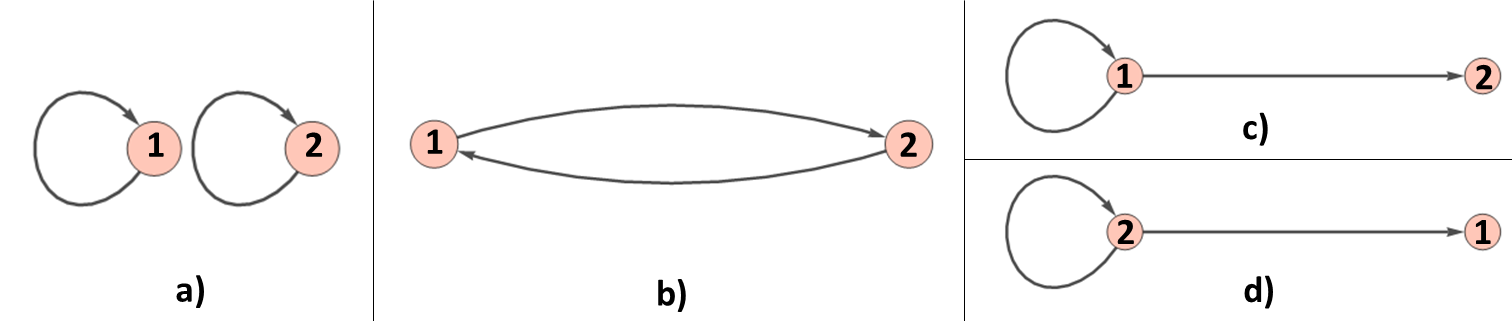
\includegraphics[width=\textwidth]{topologies}
	\caption[An ensemble of possible topologies for a Random Boolean Network.]{Ensemble of possible topologies for $N=2$ and $k=1$. The topologies a) and b) have the same statistical weight $1/4$. The topologies c) and d) are the same (we consider unlabeled digraphs) so its probability is $1/2$. If we would have assigned updating functions to the nodes, though the topologies of c) and d) are the same their updating functions would not have been necessarily the same.}
	\label{fig:topologies}
\end{figure}

The topologies generated by this model are known as \textit{homogeneous random topologies} because in the thermodynamic limit $N \rightarrow \infty$, the number of outgoing links, i.e., the vertex out-degree $ d^{+}$ of each node follows a Poisson distribution \cite{rbn_barbara}:

\begin{equation}
\label{standard_distribution}
  P_{out}(d^{+})=\frac{k^{d^{+}}}{d^{+} !} e^{-k}
\end{equation}

This means that every element of the network is statistically equivalent to any other, thus, we can characterize the topology of the network by the average connectivity $k$, as we can expect all the nodes to have a connectivity value close to this value \cite{rbn_aldana}. Nonetheless, the reader must have in mind that the probability distribution of Eq. \ref{standard_distribution} is not the only possible type of distribution which can be used to generate the topology. In fact, we could use any other probability distribution to generate the topology of the network. For instance, one of the most famous topologies is the so-called \textit{scale-free topology}\footnote{Compare with the scale-free graphs described in Section \ref{Barabasi-Albert}.} which considers the habitual feature of complex networks of having few elements with many links and many elements with few links \cite{rbn_carlos}. This type of behavior is present in molecular networks, genetic networks, social networks, etc. and is generated by the following probability distribution \cite{rbn_aldana}:

\begin{equation}
  P_{out}(d^{+})=[\zeta (\gamma) (d^{+})^{\gamma} ]^{-1}
\end{equation}

Where $\gamma >1$ and $\zeta (\gamma)= \sum_{j=1}^{\infty} j^{-\gamma}$ is the Riemann Zeta function. This time the parameter which will characterize the topology will be the scale-free exponent $\gamma$ \cite{rbn_aldana}. Throughout this work, we will not consider Boolean Networks with scale-free topologies or topologies with a probability distribution different to the probability distribution given by Eq. \ref{standard_distribution}.

\subsection{Updating Functions}
\subsubsection{Boolean Functions}
The two possible states of each node in an RBN are Boolean values, i.e., $\sigma_{i} \in \{0,1 \}$. These states are updated by means of an updating function, i.e., a logic function, Boolean function or Boolean expression which output is another Boolean value which depends in the $k$ Boolean variables used as inputs:

\begin{equation}
  f: \{0,1 \}^{k} \rightarrow \{0,1 \}
\end{equation}

Thus, an alternative definition to Eq. \ref{Boolean_function} and \ref{Boolean_function2} for a Boolean Network and which highlights it as a function is as follows \cite{coding_boolean}:\\

\begin{defn}[Alternative Definition]
\label{Alternative_Definition}
	A Boolean network of $N$ nodes can be seen as a Boolean function:

\begin{equation}
  f: \{0,1 \}^{N} \rightarrow \{0,1 \}^{N}
\end{equation}

	where $f= \{ f_{1},f_{2},...,f_{N} \}^{T}$ and each $f_{i}$ is of the form shown in Eq. \ref{Boolean_function}.\\
\end{defn}

Now, we must know how to represent the functions $f_{i}$. The easiest way to describe a Boolean function is through a truth table which is (\cite{digital}, page 26):

\begin{defn}[Truth Table]
	A list of all possible input states to a Boolean function, listed in ascending binary order, and the output response for each input combination.
\end{defn}

It can be easily seen that there are $2^{k}$ possible input states and therefore there are $2^{2^{k}}$ possible  Boolean functions for a given $k$. For instance, for $k=2$ there are $2^{2}=4$ possible input states and $2^{2^{2}}=16$ possible logic functions. The truth table for $k=2$ is shown in Table \ref{tab:truth_table}.\\

\begin{table}[t]
\centering
\begin{tabular}{ |c||c|c|c|c|c|c|c|c|c|c|c|c|c|c|c|c| } 
 \hline
 $\sigma_{1}$	$\sigma_{2}$ & $f_{0}$ & $f_{1}$ & $f_{2}$ & $f_{3}$ & $f_{4}$ & $f_{5}$ &$f_{6}$ &$f_{7}$ &$f_{8}$ &$f_{9}$ &$f_{10}$ &$f_{11}$ &$f_{12}$ &$f_{13}$ &$f_{14}$ &$f_{15}$ \\ 
 \hline
 \hline
 0	0 & 0& 0& 0& 0& 0& 0& 0& 0& 1& 1& 1& 1& 1& 1& 1& 1\\ 
 \hline
 0	1 & 0& 0& 0& 0& 1& 1& 1& 1& 0& 0& 0& 0& 1& 1& 1& 1\\
 \hline
 1	0 & 0& 0& 1& 1& 0& 0& 1& 1& 0& 0& 1& 1& 0& 0& 1& 1\\
 \hline
 1	1 & 0& 1& 0& 1& 0& 1& 0& 1& 0& 1& 0& 1& 0& 1& 0& 1\\
 \hline
\end{tabular}
 \caption{Truth table with all the possible Boolean functions for $k=2$.}
 \label{tab:truth_table}
\end{table}

Some Boolean functions receive a special name and symbol which was inherited from their use in digital electronics where they are better known as gates. We will review some of these special logic functions since they are the Lego bricks to build more complex Boolean functions.\\ 

The first of these functions is the NOT function which is usually represented as $! \sigma$, $ \neg \sigma$, $\bar{\sigma}$ or $\sim \sigma$ \cite{gates}. The truth table of this logic function is shown in Table \ref{tab:not_table}.

\begin{table}[h]
\centering
\begin{tabular}{ |c||c| } 
 \hline
 $\sigma$ & $! \sigma$\\ 
 \hline
 \hline
 0	& 1\\ 
 \hline
 1	& 0\\
 \hline
\end{tabular}
 \caption{Truth table for the NOT function.}
 \label{tab:not_table}
\end{table}

The next function is the AND function, which is usually represented as $\sigma_{1} \wedge \sigma_{2}$, $\sigma_{1} \cdot \sigma_{2}$, $\sigma_{1} . \sigma_{2}$, $\sigma_{1} \sigma_{2}$, $\sigma_{1} \& \sigma_{2}$ or $\sigma_{1} \& \& \sigma_{2}$ \cite{gates}. The truth table of this logic function is shown in Table \ref{tab:and_table}.

\begin{table}[h]
\centering
\begin{tabular}{ |c||c| } 
 \hline
 $\sigma_{1}$	$\sigma_{2}$ & $\sigma_{1} \wedge \sigma_{2}$ \\ 
 \hline
 \hline
 0	0 & 0\\ 
 \hline
 0	1 & 0\\
 \hline
 1	0 & 0\\
 \hline
 1	1 & 1\\
 \hline
\end{tabular}
 \caption{Truth table for the AND function.}
 \label{tab:and_table}
\end{table}

Finally, we have the OR function, which is usually represented as $\sigma_{1} \vee \sigma_{2}$, $\sigma_{1} + \sigma_{2}$, $\sigma_{1} | \sigma_{2}$ or $\sigma_{1} \parallel \sigma_{2}$ \cite{gates}. The truth table of this logic function is shown in Table \ref{tab:or_table}.\\

\begin{table}[h]
\centering
\begin{tabular}{ |c||c| } 
 \hline
 $\sigma_{1}$	$\sigma_{2}$ & $\sigma_{1} \vee \sigma_{2}$ \\ 
 \hline
 \hline
 0	0 & 0\\ 
 \hline
 0	1 & 1\\
 \hline
 1	0 & 1\\
 \hline
 1	1 & 1\\
 \hline
\end{tabular}
 \caption{Truth table for the OR function.}
 \label{tab:or_table}
\end{table}

The Boolean functions AND, OR and NOT are the Lego bricks from which any other Boolean function can be built (\cite{digital}, page 34). Indeed, some other special gates are derived from these three gates: the NAND, NOR, XNOR, and XOR functions.\\

The NAND (contraction of NOT AND) function inverts the output of an AND function. It is usually represented as $\sigma_{1} \bar{\wedge} \sigma_{2}$, or $\overline{\sigma_{1} \cdot \sigma_{2}} $ \cite{gates}. The truth table of this logic function is shown in Table \ref{tab:nand_table}.

\begin{table}[h]
\centering
\begin{tabular}{ |c||c| } 
 \hline
 $\sigma_{1}$	$\sigma_{2}$ & $\sigma_{1} \bar{\wedge} \sigma_{2}$ \\ 
 \hline
 \hline
 0	0 & 1\\ 
 \hline
 0	1 & 1\\
 \hline
 1	0 & 1\\
 \hline
 1	1 & 0\\
 \hline
\end{tabular}
 \caption{Truth table for the NAND function.}
 \label{tab:nand_table}
\end{table}

The NOR (contraction of NOT OR) function inverts the output of an OR function. It is usually represented as $\sigma_{1} \bar{\vee} \sigma_{2}$, $\sigma_{1} \downarrow \sigma_{2}$, or $\overline{\sigma_{1} + \sigma_{2}} $ \cite{gates}. The truth table of this logic function is shown in Table \ref{tab:nor_table}.

\begin{table}[h]
\centering
\begin{tabular}{ |c||c| } 
 \hline
 $\sigma_{1}$	$\sigma_{2}$ & $\sigma_{1} \bar{\wedge} \sigma_{2}$ \\ 
 \hline
 \hline
 0	0 & 1\\ 
 \hline
 0	1 & 0\\
 \hline
 1	0 & 0\\
 \hline
 1	1 & 0\\
 \hline
\end{tabular}
 \caption{Truth table for the NOR function.}
 \label{tab:nor_table}
\end{table}

The XOR (contraction of exclusive OR) is usually represented as $\sigma_{1} \underline{\vee} \sigma_{2}$, or $\sigma_{1} \oplus \sigma_{2} $ \cite{gates}. The truth table of this logic function is shown in Table \ref{tab:xor_table}.

\begin{table}[h]
\centering
\begin{tabular}{ |c||c| } 
 \hline
 $\sigma_{1}$	$\sigma_{2}$ & $\sigma_{1} \oplus \sigma_{2} $ \\ 
 \hline
 \hline
 0	0 & 0\\ 
 \hline
 0	1 & 1\\
 \hline
 1	0 & 1\\
 \hline
 1	1 & 0\\
 \hline
\end{tabular}
 \caption{Truth table for the XOR function.}
 \label{tab:xor_table}
\end{table}

The XNOR (contraction of exclusive NOR) is usually represented as $\overline{\sigma_{1} \oplus \sigma_{2}} $. The truth table of this logic function is shown in Table \ref{tab:xnor_table} \cite{k_2_functions}.

\begin{table}[h]
\centering
\begin{tabular}{ |c||c| } 
 \hline
 $\sigma_{1}$	$\sigma_{2}$ & $\overline{\sigma_{1} \oplus \sigma_{2}} $ \\ 
 \hline
 \hline
 0	0 & 1\\ 
 \hline
 0	1 & 0\\
 \hline
 1	0 & 0\\
 \hline
 1	1 & 1\\
 \hline
\end{tabular}
 \caption{Truth table for the XNOR function.}
 \label{tab:xnor_table}
\end{table}

Using these derived functions, and the symbols we have introduced, we can rewrite the truth table with all the possible Boolean functions for $k=2$ as in Table \ref{tab:k_2_table}.\\

\begin{table}[h]
\centering
\begin{tabular}{ |c||c| } 
 \hline
 Function & Symbol  \\ 
 \hline
 \hline
 $f_{0}$ & 0\\ 
 \hline
 $f_{1}$ & $\sigma_{1} \wedge \sigma_{2}$\\ 
 \hline
 $f_{2}$ & $\sigma_{1} \wedge ! \sigma_{2}$\\ 
 \hline
 $f_{3}$ & $\sigma_{1}$\\ 
 \hline
 $f_{4}$ & $! \sigma_{1} \wedge ! \sigma_{2}$\\ 
 \hline
 $f_{5}$ & $\sigma_{2}$\\ 
 \hline
 $f_{6}$ & $\sigma_{1} \oplus \sigma_{2} $\\ 
 \hline
 $f_{7}$ & $\sigma_{1} \vee \sigma_{2}$\\ 
 \hline
 $f_{8}$ & $\sigma_{1} \bar{\wedge} \sigma_{2}$\\ 
 \hline
 $f_{9}$ & $\overline{\sigma_{1} \oplus \sigma_{2}} $\\ 
 \hline
 $f_{10}$ & $! \sigma_{2}$\\ 
 \hline
 $f_{11}$ & $\sigma_{1} \vee ! \sigma_{2}$\\ 
 \hline
 $f_{12}$ & $! \sigma_{1}$\\ 
 \hline
 $f_{13}$ & $! \sigma_{1} \vee \sigma_{2}$\\ 
 \hline
 $f_{14}$ & $\sigma_{1} \bar{\wedge} \sigma_{2}$\\ 
 \hline
 $f_{15}$ & 1\\ 
 \hline
\end{tabular}
 \caption{Truth table with all the possible Boolean functions for $k=2$ rewritten by using symbols.}
 \label{tab:k_2_table}
\end{table}

The reader must had noticed up to this point that logic functions can be written as different compositions of distinct functions, for instance, $((\sigma_{1} \& \& ! \sigma_{2})||(! \sigma_{1} \& \& \sigma_{2}))$ and $((! \sigma_{1} || ! \sigma_{2})\& \&( \sigma_{1} || \sigma_{2}))$ are equivalent ways of representing the function $\sigma_{1} \oplus \sigma_{2} $, since all of them share the same truth table. 
One question arises: is there any preferred combination of functions when trying to represent a Boolean function besides its Boolean table? The answer will depend on the context, in general, the preferred representation will rely on our needs. However, we must know that between the derived functions we talked about above two of them highlight: the NAND and the NOR functions. These functions are known as universal logic gates since any other logic function can be implemented using only combinations of one of these functions \cite{universal_gate}. We will use this property in chapter 5 to represent Boolean functions in a systematic way, so we define:

\begin{defn}[Universal Boolean Functions]
\label{Universal_Boolean_Functions}
	The NAND and NOR functions are universal Boolean functions since any other Boolean function can be represented just by combinations of one of them.
\end{defn}

Therefore, we only need to use repeatedly one of these functions to build any other logic function.

\subsubsection{Choosing the Updating Functions}
\label{functions}
There are diverse ways to choose the set of functions for a Boolean Network, i.e., the function assigned to each node. Some techniques try to give biological meaning to this assignment (see \cite{rbn_barbara}). For example, one usual technique which tries to resemble the behavior of neural networks is that in which only threshold functions are used. Thus, the state of each node is given by \cite{rbn_barbara}:

\begin{equation}
\sigma_{i}(t+1) = \begin{cases}
1 &\text{if $\sum_{j=1}^{N}$ ($c_{ij}$($2\sigma_{j} +1$)+$h$) $\geq$ $0$}\\
0 &\text{else}
\end{cases}
\end{equation}

Where $c_{ij}=\pm 1$ with equal probability if the node $i$ receives an input from node $j$, otherwise $c_{ij}=0$.\\

Nevertheless, in this work, we will use standard logic functions and we will choose the Boolean functions of each node in the following way: as was said before, there are $2^{2^{k}}$ possible  Boolean functions for a given $k$ value, thus we will choose with a uniform probability distribution\footnote{More specifically it is a discrete uniform distribution.} a function from the set of possible Boolean functions for each node, this means that the probability of choosing each possible Boolean function is $1/(2^{2^{k}})$, e.g., for $k=2$ all the $16$ possible functions have the same probability of $1/16$ of being chosen in each node.\\

In the case where we assign the same function to all the nodes, we have what is known as a cellular automaton or finite state machine with random wiring. Thereby, a Boolean Network is a more general model \cite{rbn_barbara}.\\

A generalization to the original Kauffman model introduces a bias parameter $p$ when the Boolean functions are chosen  \cite{attractors}. This parameter gives the probability of the values in the truth table of being $1$ given a uniformly distributed input, and thereby the probability of being $0$ is $(1-p)$. Therefore, the probability of choosing a function with $n$ times the output value $1$ and $(M-n)$ times\footnote{Where $M=2^{k}$, i.e., the number of possible input states.} the output value $0$ is given by $p^{n}(1-p)^{M-n}$. Therefore, the method which we will use in this work to choose the logic functions is the special case with $p=1/2$, which means that all the possible functions have the same probability of being chosen \cite{rbn_barbara}.

\subsection{Counting RBNs}
\label{Counting_RBN_section}
Since the RBNs are generated in a random way it is useful to give us an idea of how many different RBN is possible to create given the number of nodes $N$ and the parameter $k$ of each digraph. First, we must remember that there are $2^{2^{k}}$ possible logic functions for a given $k$. Thus, for a digraph with $N$ nodes we can assign to each node one of these possible Boolean functions which gives \cite{coding_boolean}:

\begin{equation}
\label{number_rbn}
\underbrace{2^{2^{k}} \times 2^{2^{k}} \times \cdots \times 2^{2^{k}}}_\text{N \, Times} =2^{N \times 2^{k}}
\end{equation}

This is the number of possible RBNs once we have fixed the topology of the digraph. This number increases so fast, e.g., for $N=4$ and $k=2$ the number of possible RBNs for a given topology is $65,536$ and for $N=6$ and $k=2$ this number is $16,777,216$.

Nevertheless, we do not only assign the Boolean functions randomly, but we also wire the nodes of the digraph randomly, thus we must consider these combinations. If every node has the same vertex in-degree $ d^{-} (i) =k$, then each node has $N!/(N-k)!$ possible ordered combinations for $k$ different links \cite{rbn_barbara}. Consequently, combining this result with Eq. \ref{number_rbn} the number of possible RBNs generated randomly is:

\begin{equation}
\label{number_rbn_final}
(\frac{2^{2^{k}} N!}{(N-k)!})^{N}
\end{equation}

This number is even bigger than our initial estimation, e.g., for $N=4$ and $k=2$ the number of possible RBNs for a given topology is $1,358,954,496$ and for $N=6$ and $k=2$ this number has an order of magnitude of $10^{16}$. Hence, the universe of possible RBNs is immense and moreover there exists a very high variance in the statistical studies within this enormous set. However, it is possible to focus on representative features and extract some general properties \cite{rbn_barbara}.

\subsection{Dynamics: The State Space and Some Basic Definitions}
\label{dynamics_ex_rbn}
As was mentioned before, throughout this work, we will only consider the synchronous updating scheme, which means that the state of all the nodes is updated at the same time in a parallel way. Every node can have two possible states, thus the number of possible states for an RBN of $N$ nodes is $2^{N}$. Consequently, the number of possible initial states is also $2^{N}$. We will usually study all the possible initial states of every RBN since the dynamics of a Boolean Network is in general different depending on the initial state we have chosen. The configuration state of a Boolean Network at time $t$ can be represented by the vector \cite{bool_net}:

\begin{equation}
\sigma(t)\equiv \Sigma_{t+1}=\{\sigma_{1}(t),\sigma_{2}(t),...,\sigma_{N}(t)\}
\end{equation}

With this notation the dynamics of the system can be further abbreviated as \cite{rbn_aldana}:

\begin{equation}
\Sigma_{t+1}=\mathcal{F} [\Sigma_{t}]
\end{equation}

Where $\mathcal{F}$ represents the action of the updating functions $\{f_{1},f_{2},...,f_{N} \}$ on the configuration state $\Sigma_{t}$.\\

To visualize the dynamics of an RBN we represent its possible states in a $2^{N}$-dimensional state space where we assign to each state a point. If a state flows to another state according to the updating functions, we use a directed edge to join both states with the head of the directed edge pointing to the newer state. Therefore, the state space can be represented by means of a directed graph\footnote{The reader must not confuse the digraph which represents the topology of the Boolean Network and the digraph which represents the state space.} of $2^{N}$ nodes where the vertex out-degree $ d^{+} (i)$ of each node is $1$ (since every state has a unique successor state\footnote{It is said that the RBNs are dissipative systems \cite{rbn_carlos}.}). On the other hand, the vertex in-degree $ d^{-} (i)$ of each node is not fixed which means many states can drive to the same state.

The trajectory in state space has some features. First, because the state space is finite and the dynamics is deterministic, when starting from any initial state, eventually a state or a sequence of states will be repeated, which means we have reached an attractor \cite{rbn_carlos}:

\begin{defn}
A periodic sequence of states (which we also call cycle) is an \textit{attractor} if there are states outside the attractor that lead to it \cite{rbn_barbara}.
\end{defn}

\begin{defn}
If an attractor consists of only one state it is called a \textit{point attractor} or \textit{steady state}, but if it consists of two or more states, it is called a \textit{cycle attractor} or \textit{state cycle} \cite{attractors}.
\end{defn}

Thus, a point attractor can be visualized as a loop in the digraph representation of the state space. Some other interesting definitions are the following:

\begin{defn}
The \textit{size} or \textit{length of an attractor} is the number of different states on the attractor. \cite{rbn_barbara}.
\end{defn}

\begin{defn}
The \textit{basin of attraction} or \textit{attractor basin} of an attractor is the set of all states that eventually end up on this attractor, including the attractor states themselves. The \textit{size of the basin of attraction} is the number of states belonging to it.
\end{defn}

Those states which are not reachable beginning from any other state are called garden-of-Eden states:

\begin{defn}
States without predecessors are called \textit{garden-of-Eden states} \cite{rbn_carlos}.
\end{defn}

The dynamics flows from these garden-of-Eden states and converges in an attractor:

\begin{defn}
The time it takes to reach an attractor is called \textit{transient time}  \cite{rbn_carlos}.
\end{defn}


Now, it is time to see a Boolean Network in action. We will study a network of $N=4$ nodes with parameter $k=2$. The truth table for the functions in each node is shown in Table \ref{tab:example}. The digraph used in our example is shown in Fig. \ref{fig:di_example}. Now, once we have established the topology and the dynamical rules, our Boolean Network is entirely described, and its state space can be seen in \ref{fig:rbn_example}. Note that, to label the nodes in the state space diagram we have replaced the states $\{0000,0001,\cdots,1111 \}$ by their corresponding decimal representation $\{0,1,\cdots,15\}$. This convention allows us to abbreviate and make more understandable our diagram, especially when dealing with large state spaces.

\begin{table}[h]
\centering
\begin{tabular}{ |c||c|c|c|c| } 
 \hline
 $\sigma_{1}$	$\sigma_{2}$ & $f_{Node 1}$ & $f_{Node 2}$ & $f_{Node 3}$ & $f_{Node 4}$ \\ 
 \hline
 \hline
 0	0 & 1& 1& 0& 1\\ 
 \hline
 0	1 & 1& 1& 1& 1\\
 \hline
 1	0 & 0& 0& 1& 0\\
 \hline
 1	1 & 0& 1& 0& 0\\
 \hline
\end{tabular}
 \caption[Truth table with the functions assigned to a Boolean Network of $4$ nodes and parameter $k=2$.]{Truth table with the functions assigned to a Boolean Network of $4$ nodes and parameter $k=2$. These functions were chosen with a uniform probability from the set of all the possible Boolean functions of $2$ variables.}
 \label{tab:example}
\end{table}

\begin{figure}[h]
	\centering
		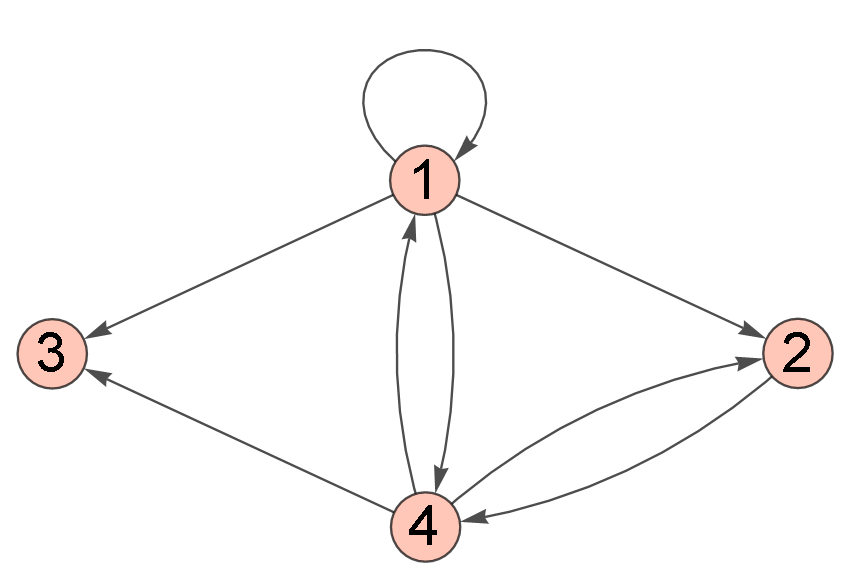
\includegraphics[scale=0.7]{di_example}
	\caption[The topology of a Boolean Network.]{Topology of a Boolean Network of $4$ nodes and vertex in-degree $2$. This topology was randomly chosen with the help of a uniform distribution among all the possible topologies with the given parameters.}
	\label{fig:di_example}
\end{figure}

\begin{figure}
	\centering
		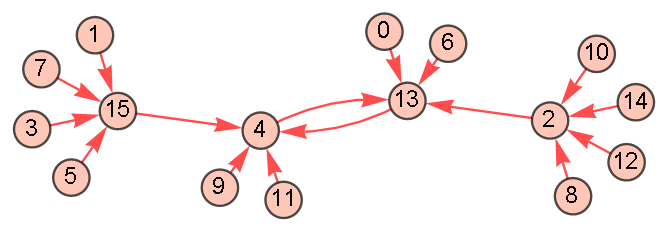
\includegraphics[width=\textwidth]{rbn_example}
	\caption[The state space of a Random Boolean Network.]{The state space of the Random Boolean Network whose topology is shown in Fig. \ref{fig:di_example} and whose dynamical rules are shown in Table \ref{tab:example}. This Boolean Network has a cycle attractor of length $2$ made up of the states $4$ and $13$. Moreover, the size of the basin of attraction is $8$ and is made up of the states $\{0,2,4,6,9,11,13,15\}$. Finally, the states $\{0,1,3,5,6,7,8,9,10,11,12,14\}$ are the garden-of-Eden states.}
	\label{fig:rbn_example}
\end{figure}

We finish this section by commenting that the study of the mean number of attractors of the RBNs is of interest, though that discussion is out of the purposes of this work.

\section{The Dynamical Phases}
Since in the end, the RBNs are dynamical systems, we can expect their dynamics will have distinct phases. To visualize them, we must plot the states of each node of the network in a grid such that every square represents a node and neighbor squares depend topologically as in the original network \cite{rbn_carlos}. If the state of a node is "on" we can color it black and if it is "off" we can color it white. Then, we choose an initial state and let the dynamics flow. In this way, it is possible to distinguish three phases with unique features: the ordered, chaotic and critical phases.\\

The \textit{ordered} or \textit{frozen phase} is characterized because when we choose a random initial state, initially many states will be changing, however, it will be stabilized quickly and most of the nodes will be static, i.e., almost all nodes are frozen. Also, in this regime attractor cycles are short \cite{attractors}. Another feature is that when we introduce small perturbations to the network, such as changing the connection between two nodes or flipping the states of a node, this damage usually will not be spread, i.e., the perturbation dies out and the behavior of the perturbed network is similar to the normal network. The final feature is that similar states tend to converge to the same state \cite{rbn_carlos}.\\

The \textit{chaotic phase} is characterized because when we choose a random initial state, states are not stabilized and most of them stay changing, i.e., states have fluctuating values. Besides, in this regime attractor cycles can be long \cite{attractors}. When we introduce small perturbations to the network this phase is highly sensitive and small changes tend to propagate through the network, i.e., perturbations have strong effects making these networks not robust\footnote{We say that a system is robust if it continues functioning after a perturbation \cite{guiding_rbn}}. This is the well-known butterfly effect which is exhibited by chaotic systems. Moreover, in this phase similar states tend to diverge \cite{rbn_carlos}.\\

The \textit{critical phase} is at the border between the ordered and chaotic phases \cite{rbn_barbara}. Between these two phases occurs a phase transition called the \textit{edge of chaos}. At this transition phase, perturbations can propagate, though not necessarily through all the network. Besides, similar states perform a trajectory that neither diverges nor converges \cite{rbn_carlos}. The networks within this regime are of biological interest because it is thought they are complex enough to allow biological processes but also flexible enough to deal with changes \cite{attractors}.\\

Apart from the visualization approach, there exist methods more standard to identify these phase transitions. The idea behind them is to measure the effect of perturbations, the sensitivity to initial conditions, or the damage spreading \cite{rbn_carlos}, i.e., the main idea is to distinguish the features of each phase by computing some statistical or analytical measurements. 

It is known that in the limit $N\rightarrow \infty$ the phases are controlled by the parameter $k$ and the bias parameter $p$ we mentioned in Section \ref{functions} \cite{attractors}. The system is chaotic for $k\cdot 2p \cdot (1-p) >1$ and ordered for $k\cdot 2p \cdot (1-p) <1$. In the uniform case $p=0.5$, we have the ordered regime for $k<2$, the chaotic regime for $k<2$ and the edge of chaos at $k=2$. In Fig. \ref{fig:critical_curve} can be seen the critical curve showing the boundary between these regimes for different values of $k$ and $p$.

\begin{figure}
	\centering
		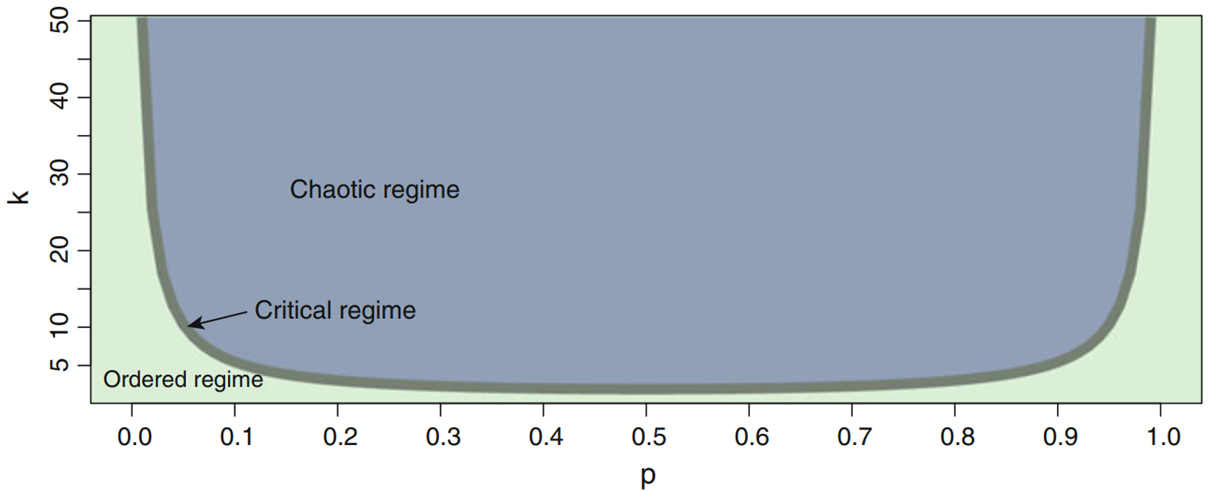
\includegraphics[width=\textwidth]{critical_curve}
	\caption[Dynamical phases of Boolean Networks.]{The critical curve which shows the border between the chaotic and ordered regimes as a function of the parameters $k$ and $p$. Reprinted from \cite{attractors} by permission from Springer Nature (adapted from \cite{rbn_aldana} by permission from Elsevier).}
	\label{fig:critical_curve}
\end{figure}

Though we will not delve into the subject and we will not further analyze the properties of these phases, we can mention, for instance, that for critical networks with parameter $k=2$ and $N$ nodes Kauffman originally found by computer simulations that the number of attractors goes as $\sqrt{N}$, although more recently it was shown that this number grows greater than any power law with $N$, i.e., it grows superpolynomially \cite{attractors}. Meanwhile, in scale-free topologies, the transition from order to chaos occurs at the vale of the exponent $\gamma_{c}$ which solves the transcendental equation \cite{rbn_aldana}:

\begin{equation}
2p(1-p) \frac{\zeta (\gamma_{c -1})}{\zeta (\gamma_{c})}=1
\end{equation}

\section{Other Updating Schemes}
Coming back to the original paper of Kauffman, he focused his study on critical networks since as we argued before, they seem to be more robust to the life features. It is well known that different type cells from the same individual share the exact same genetic information, but they differ in their genetic activity, which differentiates them. In this way, Kauffman thought that having the same DNA equals to having the same network, i.e., each gene is a node of a network and thereby its number of attractors must be equal to the number of different cell types and the attractor's length to the cell cycle time \cite{rbn_barbara}. As we mentioned, he found that the average number of attractors and their length was proportional to $\sqrt{N}$. He argued that the number of attractors found in the RBNs compared with the number of possible states is analogous to the number of cell types compared with the number of genes \cite{rbn_carlos}. His idea was backed because in those years available data pointed out that the number of cell types seems to be proportional to the square root of the number of genes for distinct species \cite{rbn_barbara}. At that time, the number of genes which forms the human genome was believed to be around $8000$, thus agreeing with the number of human cell types \cite{rbn_carlos}. Nevertheless, once the Human Genome Project sequenced human DNA, we knew it consists of around $25,000$ genes (\cite{human_genome}, page 1239). This discrepancy is due mainly\footnote{Among other loopholes of this model, we can cite: the lack of consideration of scale-free topology and biased functions and the existence of non-coding DNA without any functionality \cite{rbn_carlos}.} to the assumption of synchronicity in the genes' activity. There is no reason to think genes change their state at the same time. Some genes change their state before others, i.e., their dynamics is asynchronous \cite{rbn_carlos}.\\

As was said at the beginning, the updating scheme which we will be considering is synchronous, which means states of nodes at time $t+1$ are determined by states of nodes at time $t$, so states in all the nodes must be updated at the same time. However, this model is not realistic, so for the sake of completeness, we will briefly define some variations which can be introduced to the original $N-k$ model by means of different updating schemes. We will name the original Kauffman network model as \textit{Classical Random Boolean Networks (CRBN)}.

\subsection{Asynchronous RBNs}
In the \textit{Asynchronous  Random Boolean Networks (ARBNs)}, unlike CRBNs, at each step, only one randomly chosen node is updated. This asynchronous updating destroys the deterministic behavior of the network. There are no cycle attractors only point attractors can exist, though once the system falls into a point attractor it cannot escape from it. Also, there exist \textit{loose attractors}, which are regions of the state space which capture the dynamics of the network, even though their order is not repeated deterministically due to the random updating order of the nodes \cite{updating_scheme1}.

\subsection{Generalized Asynchronous RBNs}
The \textit{Generalized Asynchronous Random Boolean Networks (GARBNs)} are a generalization of the ARBNs. In this model, at each step, the nodes to be updated are chosen randomly, i.e., unlike ARBNs, in the GARBNs the number of randomly chosen nodes to be updated can be a number between one or all of them, even updating none is a possibility at each step. This model also is non-deterministic and lacks cycle attractors. Only point and loose attractors can exist \cite{updating_scheme2}.

\subsection{Deterministic Asynchronous RBNs}
In the model of \textit{Deterministic Asynchronous Random Boolean Networks (DARBNs)}, we associate two parameters to each node: $p$ and $q$ such that $p$,$q\in \mathbb{N}$ and $q<p$. These parameters control the frequency of the update of each node. If the modulus of $p$ over time equals $q$, then the node is updated. If two or more nodes are to be updated at the same step, then they are updated one after the other in an arbitrary order. This model does allow the existence of both point and cycle attractors, allowing the model of asynchronous but not random phenomena \cite{updating_scheme1}.

\subsection{Deterministic Generalized Asynchronous RBNs}
The model of \textit{Deterministic Generalized Asynchronous Random Boolean Networks (DGARBNs)} is like the model of DARBNs, with the difference that nodes are updated if they fulfill the condition $(p\,mod\,t)==q$ and there is no arbitrary restriction to update them one after the other because all of them are updated at the same time, i.e., in a synchronous way \cite{updating_scheme2}.

\subsection{Mixed-context RBNs}
The \textit{Mixed-context Random Boolean Networks (MxRBNs)} are like the DGARBNs, with the difference that each $T$ time steps the values of $p$ and $q$ are randomly chosen from the sets $\bar{P}$ and $\bar{Q}$. These sets contain different values for $p$ and $q$ respectively which are called the contexts of the network \cite{updating_scheme2}.\\

All the random Boolean Networks previously discussed are classified as \textit{Discrete Dynamical Networks (DDN's)} since they all have discrete-time, states, and values \cite{updating_scheme1}. A diagram showing the classification of the RBNs discussed in this section can be seen in Fig. \ref{fig:rbn_classification}. The model of DDN's includes the \textit{Multi-Valued Networks} in which nodes can take more than two discrete values (if they were continuous, they would be real-valued networks which study is up to dynamical systems theory)\cite{updating_scheme1}.

\begin{figure}
	\centering
		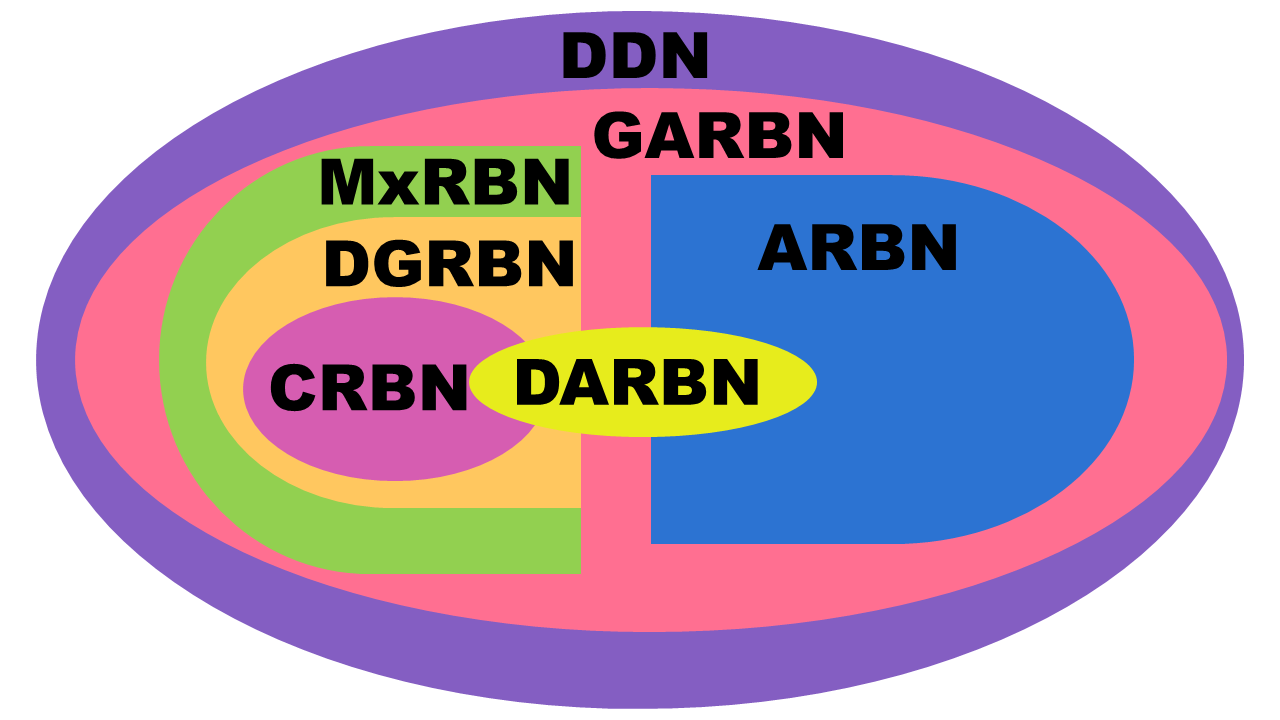
\includegraphics[scale=0.4]{rbn_classification}
	\caption[Classification of Random Boolean Networks according to their updating scheme.]{Classification of Random Boolean Networks according to their updating scheme \cite{updating_scheme1}.}
	\label{fig:rbn_classification}
\end{figure}

\section{Applications of The RBNs}
\label{Applications_RBN}
As we have mentioned, Random Boolean Networks were originally conceived by Kauffman as an abstract model of gene regulatory networks. Using these networks, we can model the causal link between genes by means of a directed edge, the expression or not expression of a gene by assigning to them a Boolean value, or even the stability of the cell (to damage, mutations, etc.) by means of the examination of  the sensibility of attractors to perturbations, like a change in the network topology, a change in an updating function, a change in the state of a node, etc \cite{kauffman_analysis_applications}. In this sense, Random Boolean Networks have been used to study the transcriptional network and the network regulating the cell cycle in the budding yeast \textit{Saccharomyces cerevisiae} \cite{yeast_rbn_kauffman} \cite{yeast_rbn}. The use of \textit{Saccharomyces cerevisiae} had a great advantage because it is an organism well studied and thereby, we know or have an idea about the topologies of its regulation networks. If we know the topology of the network, half of our work is done, and we only must vary the random updating functions. Nevertheless, even if the topology is unknown, it is possible to infer it by means of experimental data (see \cite{model_construction_rbn}). When the genetic data is incomplete or insufficient, then \textit{probabilistic Boolean Networks} are usually used \cite{rbn_carlos}. The objective of modeling genetic networks with RBNs is to describe regulations at a system level, analyze and predict genomic interactions but also intervene in the network \cite{tutorial_rbn}. For instance, with the current knowledge about protein-protein interactions in cancer, it was possible to develop a topology to evaluate by means of the RBNs some possible molecularly targeted cancer therapies \cite{cancer_rbn}. Among other applications of the RBNs to genetic modeling, we can cite the study of the cell cycle of the fission yeast \textit{S. pombe} \cite{prospects_rbn}, the prediction of the expression pattern of the segment polarity genes in \textit{Drosophila melanogaster} \cite{drosophila_rbn}, the analysis of the mammalian cell cycle \cite{mammalian_rbn}, etc.\\

Nonetheless, the field of application of the RBNs is not restricted to genetic networks. It has also been applied for example, to the study of Neural Networks \cite{neural_rbn}, social segregation modeling \cite{social_rbn}, music generation \cite{music_rbn}, statistical physics \cite{spin_rbn}, and due to the robustness and rich dynamics of the critical RBNs, their study represents an abstract study of the evolution of life \cite{guiding_rbn}. Even an application to implement logic functions by Kauffman networks has been proposed \cite{kauffman_analysis_applications}. Since the RBNs are a generalization of cellular automata, the number of possible applications is immense. Even though the RBNs could represent only a first step to the more realistic modeling of real-world networks, they already have proved to be of value in several different areas.

\section{Software to Study RBNs}
To study the properties, visualize the dynamics and simulate in an easy way the RBNs, we can resort to \textit{The BoolNet R} package \cite{attractors} or to \textit{The PyBoolNet} package written for being used in python language \cite{pyboolnet}. Other software tools are \textit{The DDLab}, \textit{The RBNLab}, and the Matblab implementations \textit{RBN Toolbox} and \textit{BN/PBN Toolbox} \cite{rbn_carlos}.\\

Despite the existence of different software implementations to study the RBNs for various platforms, in the next chapters, we will use our own algorithms. This will allow us to better understand the functioning of the RBNs. Moreover, since we are only interested in the study of a few properties of the Random Boolean Networks, the creation of our own algorithms will enable us to focus on the features we need with the advantage that it is easier to debug the code that we have written ourselves. This flexibility does not exist when we use the software created by anyone else and we must adapt our needs to whatever the program offers us.
What is more, these algorithms will be developed in the Wolfram Language, a powerful platform for which we have not found any implementation to analyze Boolean Networks. The algorithms used throughout this work to study the RBNs are presented at the end, in the Appendix section.